\documentclass{article}
\usepackage{graphicx}
\graphicspath{ {./images/} }
\begin{document}
    
%Header
\begin{flushleft}
    Evan Wilcox\\
    CS1200 Fall 2018\\
    Homework 4\\
    Due: Monday 10/22/18
\end{flushleft}
    
%Problems
\begin{enumerate}

    %1
    \item Using truth tables, prove the following arguments are valid.
    \begin{enumerate}
        
        %a
        \item 
        \begin{tabular}{ |c|c|c|c|c|c|c| }
            \hline
            $P$ & $Q$ & $R$ & $P \rightarrow \sim Q$ & $\sim R|Q$ & $R$ & $\sim P$\\
            \hline
            F & F & F & T & T & F & T\\
            \hline
            F & F & T & T & F & T & T\\
            \hline
            F & T & F & T & T & F & T\\
            \hline
            F & T & T & T & T & T & T\\
            \hline
            T & F & F & T & T & F & F\\
            \hline
            T & F & T & T & F & T & F\\
            \hline
            T & T & F & F & T & F & F\\
            \hline
            T & T & T & F & T & T & F\\
            \hline
        \end{tabular}

        %b
        \item 
        \begin{tabular}{ |c|c|c|c|c|c| }
            \hline
            $P$ & $Q$ & $R$ & $P \rightarrow Q$ & $Q \rightarrow R$ & $P \rightarrow R$\\
            \hline
            F & F & F & T & T & T\\
            \hline
            F & F & T & T & T & T\\
            \hline
            F & T & F & T & F & T\\
            \hline
            F & T & T & T & T & T\\
            \hline
            T & F & F & F & T & F\\
            \hline
            T & F & T & F & T & T\\
            \hline
            T & T & F & T & F & F\\
            \hline
            T & T & T & T & T & T\\
            \hline
        \end{tabular}
        
    \end{enumerate}

    
    %2
    \item Use Python programs to verify the results in Problem 1.

    \begin{enumerate}
        \item Python code for part a.\\
        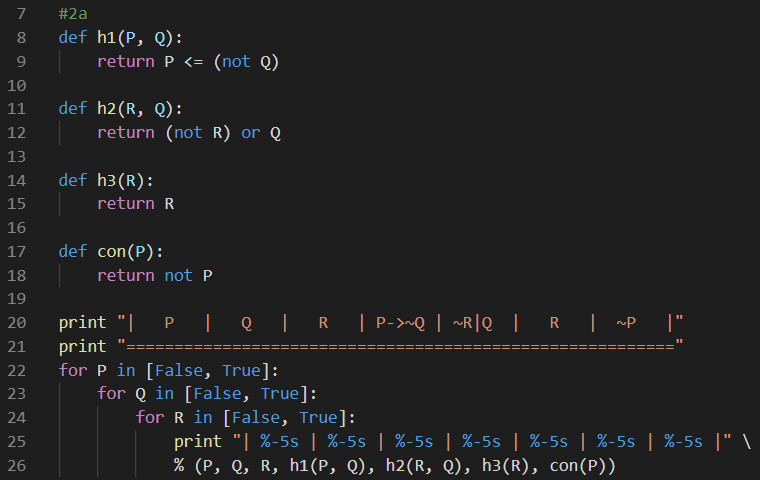
\includegraphics[scale=.6]{2a1}\\
        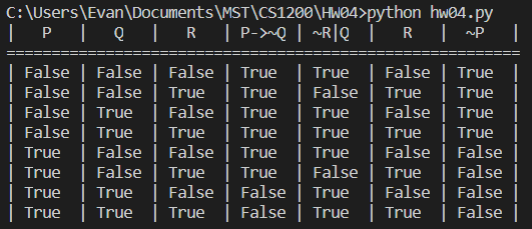
\includegraphics[scale=.7]{2a2}
        \item Python code for part b.\\
        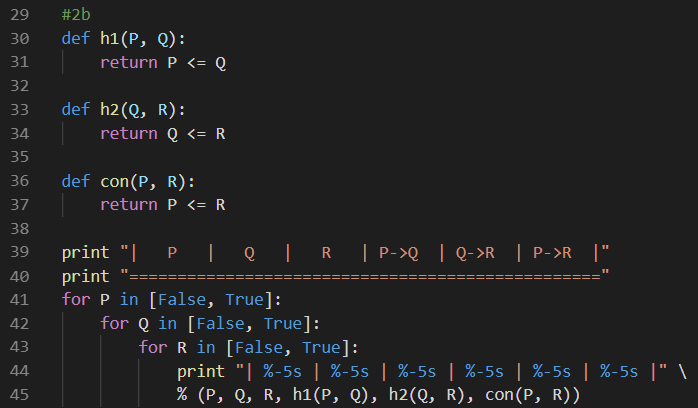
\includegraphics[scale=.6]{2b1}\\
        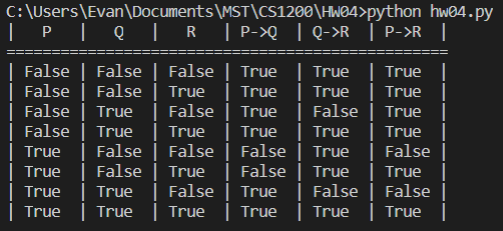
\includegraphics[scale=.7]{2b2}
    \end{enumerate}

    %3
    \item Derive the associated sets for the arguments in Problem 1.
     
    \begin{enumerate}
        \item The set $[\sim Q, Q, R, P]$ is not satisfiable, so the argument is valid.
        
        \begin{tabular}{ p{4cm} p{4cm} p{4cm}}
            $P \rightarrow \sim Q$ & $\sim P |\sim Q$ & $\sim Q$\\
            $\sim R|Q$             & $\sim R|Q$       & $Q$\\
            $R$                    & $R$              & $R$\\
            $\sim (\sim P)$        & $P$              & $P$
        \end{tabular}
        
        \vspace{10px}
        
        \item The set $[Q, \sim Q, P, \sim R]$ is not satisfiable, so the argument is valid.
        
        \begin{tabular}{ p{2.5cm} p{2.5cm} p{2.5cm} p{2.5cm}}
            $P \rightarrow Q$       & $\sim P |Q$       & $\sim P|Q$    & $Q$\\
            $Q \rightarrow R$       & $\sim Q|R$        & $\sim Q|R$    & $\sim Q$\\
            $\sim(P \rightarrow R)$ & $\sim (\sim P|R)$ & $P \& \sim R$ & $P$\\ 
                                    &                   &               & $\sim R$
        \end{tabular}
    \end{enumerate}


    \newpage
    %4
    \item 
    \begin{enumerate}

        %a
        \item Neither $[\sim P, \sim Q, P]$ or $[Q, \sim Q, P]$ are satisfiable so the argument is valid.
        \begin{center}
        \setlength{\tabcolsep}{10pt}
        \centering
        \begin{tabular}{ p{1.2cm}|p{1.1cm}|p{1cm}|p{1cm}}
        
            Start & A & A.1 & A.2\\
            \hline
            $P \rightarrow Q$ & $\sim P |Q$ & $\sim P$    & $Q$\\
            $\sim Q$          & $\sim Q$    & $\sim Q$    & $\sim Q$\\ \cline{1-1}
            $\sim P$          & $P$         & $P$         & $P$\\
        \end{tabular}
        \end{center}

        \vspace{20px}
        \begin{enumerate}
            \item $\sim P|Q$ splits A into A.1 and A.2. 
        \end{enumerate}
        
        \vspace{100px}
        
        %b
        \item Neither B.1, B.2, C.1 or C.2 are satisfiable so the argument is valid.
        \begin{center}
        \setlength{\tabcolsep}{10pt}
        \centering
        \begin{tabular}{ p{1.4cm}|p{1.5cm}|p{1cm}|p{1cm}}
            
            Start & A & B & C\\
            \hline
            $P \rightarrow \sim Q$ & $\sim P |\sim Q$ & $\sim P$    & $\sim Q$\\
            $Q|R$                  & $Q|R$            & $Q|R$    & $Q|R$\\ 
            $P$                    & $P$              & $P$         & $P$\\ \cline{1-1}
            $R$                    & $\sim R$         & $\sim R$          & $\sim R$\\
        \end{tabular}
        \end{center}

        \begin{center}
            \setlength{\tabcolsep}{10pt}
            \centering
            \begin{tabular}{ p{1cm}|p{1cm}|p{1cm}|p{1cm} }
                B.1 & B.2 & C.1 & C.2\\
                \hline
                $\sim P$ & $\sim P$ & $\sim Q$ & $\sim Q$\\
                $Q$      & $R$      & $Q$      & $R$\\ 
                $P$      & $P$      & $P$      & $P$\\
                $\sim R$ & $\sim R$ & $\sim R$ & $\sim R$\\
            \end{tabular}
        \end{center}

            \vspace{20px}
            \begin{enumerate}
                \item $\sim P| \sim Q$ splits A into B and C. 
                \item $Q|R$ splits B into B.1 and B.2.
                \item $Q|R$ splits C into C.1 and C.2.
            \end{enumerate}

    \end{enumerate}

    \newpage
    %5
    \item Translate the argument into symbolic form and use the
    truth tree method to decide if the argument is valid.

    \fbox{\begin{minipage}{12em}
        $(M \& C) \rightarrow (\sim S|H)$\\
        $(\sim C|S) \rightarrow (\sim M \& \sim H)$\\
        $(\sim M \rightarrow C) | (\sim S \rightarrow H)$
        \par\noindent\rule{\textwidth}{0.4pt}
        $(M|S) \rightarrow (C\& \sim H)$
    \end{minipage}}


    \begin{tabular}{ p{12em} p{12em} p{15em}}
        $(M \& C) \rightarrow (\sim S|H)$ & $\sim(M \& C) | (\sim S|H)$ & $\sim M | \sim C | \sim S|H$\\
        $(\sim C|S) \rightarrow (\sim M \& \sim H)$ & $\sim(\sim C|S)) | (\sim M \& \sim H)$ & $(C \& \sim S) | (\sim M \& \sim H)$\\ 
        $(\sim M \rightarrow C) | (\sim S \rightarrow H)$ & $(\sim(\sim M) | C) | (\sim(\sim S) | H)$ & $M | C | S | H$\\
        $\sim ((M|S) \rightarrow (C\& \sim H))$ & $\sim (\sim(M|S) | (C\& \sim H))$ & $\sim ((\sim M \& \sim S) | (C\& \sim H))$\\
    \end{tabular}

    \vspace{10px}

    \begin{tabular}{ p{14em} p{12em} p{15em}}
        $\sim M | \sim C | \sim S|H$ & $\sim M | \sim C | \sim S|H$ & $\sim M | \sim C | \sim S|H$\\
        $(C \& \sim S) | (\sim M \& \sim H)$ & $(C \& \sim S) | (\sim M \& \sim H)$ & $(C \& \sim S) | (\sim M \& \sim H)$\\ 
        $M | C | S | H$ & $M | C | S | H$ & $M | C | S | H$\\
        $\sim (\sim M \& \sim S) \& \sim(C\& \sim H))$ & $(M | S) \& (\sim C | H)$ & $(M | S)$\\
         &  & $(\sim C | H)$\\
    \end{tabular}

    \vspace{10px}

    \begin{tabular}{ c| p{11em} c| p{6em} c| p{6em}}
        1. & $\sim M | \sim C | \sim S|H$         & 1.  & $\sim C*$           & 1.  & $\sim C$\\
        2. & $(C \& \sim S) | (\sim M \& \sim H)$ & 2.  & $\sim M \& \sim H$ & 2a. & $\sim M$\\ 
        3. & $M | C | S | H$                      & 3.  & $M | C | S | H$    & 2b. & $\sim H$\\
        4. & $M | S$                              & 4.  & $M | S$            & 3.  & $S$\\
        5. & $\sim C | H$                         & 5a. & $\sim C$           & 4.  & $S$\\
           &                                      &     &                    & 5a. & $\sim C$\\
    \end{tabular}

    \vspace{10px}
    \par\noindent\rule{\textwidth}{0.4pt}
    \vspace{3px}

    \begin{tabular}{ c| p{11em} c| p{6em} c| p{12em}}
        1. & $\sim M | \sim C | \sim S|H$         & 1.  & $H*$             & 1.  & $H$\\
        2. & $(C \& \sim S) | (\sim M \& \sim H)$ & 2.  & $C \& \sim S$   & 2a. & $C$\\ 
        3. & $M | C | S | H$                      & 3.  & $H*$            & 2b. & $\sim S$\\ 
        4. & $M | S$                              & 4.  & $M | S$         & 3.  & $H$\\
        5. & $\sim C | H$                         & 5b. & $H$             & 4.  & $M*$\\
           &                                      &     &                 & 5a. & $H$\\
    \end{tabular}

    \vspace{10px}

    The argument is not valid. $[\sim M, \sim C, S, \sim H]$ and $[M, C, \sim S, H]$ are counter examples.

    \newpage
    %6
    \item Write Python functions to solve the problem.

    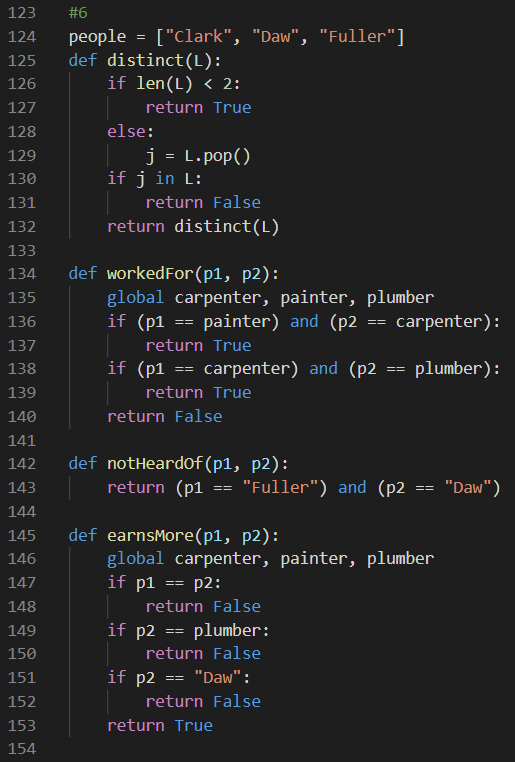
\includegraphics[scale=.7]{6a}\\
    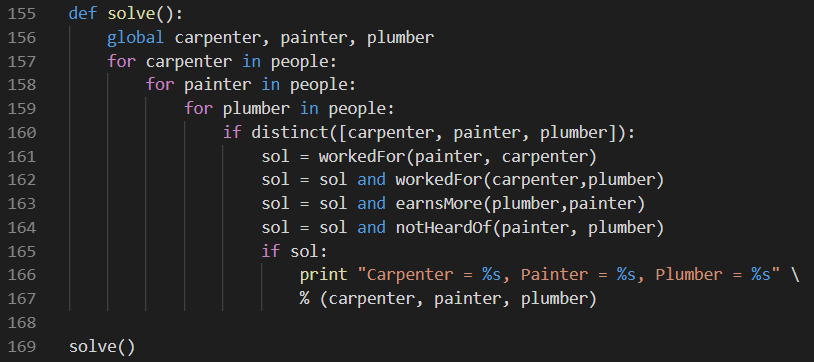
\includegraphics[scale=.7]{6b}\\
    
\includegraphics[scale=.8]{6c}

    \newpage
    %7
    \item Indicate whether each of the following predicates is true or false, 
    and give a brief justification for each answer.
    
    \begin{tabular}{ |c|c|p{60mm}| }
        \hline
        Predicate                       & True or False? & Why?\\
        \hline
        $\forall$A $\forall$B PRED(A,B) & False          & If A = 0 and B = 1, then the predicate is false.\\
        \hline
        $\forall$A $\exists$B PRED(A,B) & False          & There is no value of B that makes the predicate true for all values of A.\\
        \hline
        $\exists$A $\forall$B PRED(A,B) & False          & There is no value of A that makes the predicate true for all values of B.\\
        \hline
        $\exists$A $\exists$B PRED(A,B) & True           & If A = 1 and B = -1, then the predicate is true.\\
        \hline
    \end{tabular}

\end{enumerate}





\end{document}
